\documentclass[11pt,letterpaper]{article}

\usepackage[margin=1in]{geometry}
\usepackage[T1]{fontenc}
\usepackage{lmodern,microtype,setspace}
\usepackage{amsmath,amssymb,amsthm}
\usepackage{booktabs}
\usepackage{array}
\usepackage{tabularx}
\usepackage[round,authoryear]{natbib}
\setcitestyle{aysep={}}
\usepackage[hidelinks]{hyperref}
\usepackage{tikz}
\usepackage{pgfplots}
\pgfplotsset{compat=1.18}

\newtheorem{theorem}{Theorem}
\newtheorem{lemma}{Lemma}
\newtheorem{corollary}{Corollary}

\title{A Single Availability Date Changes the Approximability of Delay in Fixed-Order Flow Shops}
\author{}
\date{}
\hypersetup{pdftitle={A Single Availability Date Changes the Approximability of Delay in Fixed-Order Flow Shops},pdfauthor={}}

\begin{document}
\onehalfspacing
\maketitle

\begin{abstract}
We study worst-case delay in a fixed-order flow shop when a budget limits additional no-idle requirements. A machine-index anti-Monge inequality and monotone availability terms yield an exact pseudopolynomial algorithm whose budget recursion is independent of the job count after preprocessing. Even for two jobs with zero setups, one terminal availability date makes detecting a positive increase weakly NP-complete, although absolute makespan admits a fully polynomial-time approximation scheme. Subtracting an input-specified fraction of the baseline can rule out every fixed approximation factor even with strictly positive scores. A source decomposition yields a relative approximation under a bound on baseline slack. Deleting all downstream availability dates admits a linear-time maximum-error test. Testing redundancy of one upstream date with a terminal date retained is weakly coNP-complete. For switched max-plus systems, a sharp projective-diameter bound controls the singleton error certificate after suffix deletion. A budget-sensitive certificate also applies to nonconsecutive deletions. Across nine fixed-order instances, machine-state scoring achieved median paired CPU speedups of 23.43 to 29.56 times at the largest tested budget, including preprocessing. Gains in time-limited permutation search remained below one percent.

\medskip
\noindent\textbf{Keywords}\enspace Flow shop scheduling, approximation algorithms, model reduction.\par
\noindent\textbf{Subject classifications}\enspace Production/scheduling, fixed-order flow shops. Dynamic programming, budgeted machine selection.\par
\noindent\textbf{Area of review}\enspace Optimization.
\end{abstract}

\section*{Introduction}

In continuous-processing flow shops such as furnaces, kilns, and setup-intensive production lines, a fixed job sequence can still be vulnerable to changes in which machines are permitted to wait between consecutive jobs. Imposing a no-idle requirement forces a machine to process the entire sequence without interruption once it starts, coupling the timing of every job on that machine. To stress-test a committed production order, we assign positive integer costs to imposing additional no-idle requirements beyond a compulsory baseline set and ask which budget-feasible subset maximizes the increase in the earliest makespan. Because a large baseline makespan can coexist with zero incremental delay, attributing disruption to the added continuity requirements demands measuring the net increase relative to the baseline schedule rather than the absolute makespan alone.

A single machine availability date can conceal that incremental delay. Consider a two-job flow shop with two optional machines. When all machines are available at time zero, requiring either machine alone to run without idle time increases the makespan by one unit, and requiring both increases it by two. Delaying only the final machine's initial availability raises the baseline makespan by one unit, so either optional requirement alone now produces zero net increase, whereas imposing both still lifts completion above the terminal floor. A screening rule based on individual machine effects misses the joint disruption completely.

At first sight, this phenomenon resembles budgeted longest-path interdiction in general project networks, where heterogeneous budgets are already known to be weakly NP-hard via knapsack reductions and a competing parallel path can mask upstream delays and break submodularity. That general-network analogy, however, misses both halves of what makes the fixed-order flow shop structurally distinctive. On the positive side, without external availability dates (or anticipatory first setups), a fixed-order mixed no-idle flow shop is strictly better behaved than a general project network: its makespan is submodular in the set of no-idle machines, positive delay is detectable in linear time by checking singletons, and the maximum net increase admits a fully polynomial-time approximation scheme (FPTAS). On the negative side, general project-network hardness does not settle whether competing-path masking can actually arise inside the rigid timing equations of a legal flow shop with fixed processing times, unlimited buffers, no parallel bypass arcs, and only two jobs.

This paper resolves both sides of that boundary and makes three distinct contributions. First, exploiting the rank-one synchronization of no-idle machines, we establish a machine-index anti-Monge inequality for homogeneous inter-machine transitions alongside predecessor monotonicity for availability-clock terms (Section~\ref{sec:recurrence}). Together they yield an exact pseudo-polynomial algorithm whose budget phase decouples the job count into a one-time preprocessing step, accelerating repeated fixed-order evaluations relative to job-position dynamic programming. Second, our two-job construction proves that the minimal departure from homogeneous timing---adding a single initial availability date on the terminal machine (or equivalently a single anticipatory setup before its first job), with zero other setups and fixed processing times---already realizes arbitrary knapsack thresholds, making positive-increase detection weakly NP-complete and ruling out every finite-factor differential approximation unless P equals NP (Section~\ref{sec:hardness}). Rather than leaving the boundary purely negative, max-plus superposition across timing sources recovers a certified relative approximation whose running time is governed by the baseline slack of an optimizing source, reducing to an FPTAS when job arrivals dominate (Section~\ref{sec:approx}). Third, the same synchronization-versus-masking mechanism governs timing-data reduction across all budget-feasible scenarios (Section~\ref{sec:deletion}): deleting all availability dates on any downstream suffix admits a linear-time maximum-error test achieved by the baseline or a single optional machine---which also certifies when the single-source FPTAS applies---whereas retaining a single terminal date makes testing the redundancy of one upstream availability date weakly coNP-complete. Operation-level availability bounds, deterministic transport lags, arbitrary clock deletion, and minimum-cardinality clock retention are developed in the Technical Appendix.

Corollary~\ref{cor:shifted} locates an approximation boundary between absolute makespan and baseline-relative delay. Absolute makespan and subtraction of any fixed fraction below one admit an FPTAS. A fraction specified in the input can make every fixed approximation factor unattainable unless P equals NP, even when every feasible shifted score is positive.

We keep the scope of our claims explicit. All theoretical guarantees fix the job sequence and assume deterministic durations, unlimited buffers, and single initial availability lower bounds; they do not cover mid-horizon outage windows, upper transfer or zero-wait constraints, or outer permutation re-optimization. Our computational study (Section~\ref{sec:computational}) uses truncated public processing-time matrices and synthetic instances rather than plant-floor data. In those fixed-order tests, machine-state scoring delivers substantial speedups for single large budgets and multi-cost sweeps, whereas embedding the same exact evaluator in time-limited permutation search yields mean worst-case makespan improvements below a prespecified one-percent threshold.

\section{Model and Relation to Earlier Work}
\label{sec:model}

Jobs $1,\ldots,n$ visit machines $1,\ldots,m$, processing in that order on every machine, with $m,n\ge 1$. Buffers are unlimited. Job $t$ becomes available at the first machine at time $r_t$. Machine $i$ is available from time $R_i$ onward. Processing times $p_i(t)$, setup times $s_i(t)$, and availability times are nonnegative integers. A setup occupies the machine and may begin before the corresponding job arrives. At a no-idle machine, setup and processing of successive jobs occupy the machine continuously from its chosen start. There are no later outages or shared setup resources. Inputs include a compulsory no-idle set $F$, optional machines with positive integer costs $w_i$, and an integer budget $B\ge 0$. All numerical inputs are binary encoded. Let $C(S)$ denote the earliest makespan when the no-idle set is $F\cup S$. We seek a feasible $S$ maximizing $\Delta(S)=C(S)-C(\varnothing)$.

\subsection{Mixed No-Idle Scheduling and Max-Plus Foundations}

The fixed-order mixed no-idle recurrence is established, as is its use inside algorithms that optimize the job permutation for a prescribed no-idle set \citep{Pan2014,Bektas2020}. Rank-one max-plus representations already explain why a no-idle machine can be collapsed to a single start time \citep{Kubo2018,Kubo2018Thesis}. Initial machine availability and anticipatory setup times have likewise been studied for permutation minimization \citep{PerezGonzalez2009,Wang2007}. Here the job sequence is fixed input and the decision variable is the budgeted set of added continuity requirements. Because $C(\varnothing)$ is the worst feasible absolute objective value in this maximization problem, a relative guarantee on $\Delta(S)$ is a differential approximation guarantee in the sense of \citet{Demange1996}.

\subsection{Distinction from General Budgeted Longest-Path Interdiction}

Budget-constrained project networks provide direct algorithmic precedents for selecting arcs or groups of arcs to lengthen a critical path \citep[][\S4]{Brown2005} and \citet{Wu2026}. When the job permutation is fixed, our problem embeds into a layered job-position DAG in which each optional machine's backward job-position arcs form an antichain group traversed at most once by any source-to-sink path; uniform layer shifting converts these transitions into nonnegative activity extensions. Generic resource-layered dynamic programming on that network therefore solves our problem in $O(mn^2(B+1))$ work, and exploiting within-machine prefix and suffix separability tightens this job-position baseline to $O(mn(B+1))$.

Rank-one synchronization collapses transitions onto candidate \emph{machine indices}. The four-point anti-Monge inequality for these intervals complements established job-level inverse-Monge results for flow-shop input--output maps \citep[][\S12]{Imaev2009}. Together with the monotone availability terms and concave Monge path-search primitives \citep{Aggarwal1994,Galil1990}, it removes the job dimension from the budget recursion after preprocessing.

A parallel path in a general project network can mask upstream delay and break submodularity of the net increase \citep{Wu2026}. For fixed-order flow shops with immediate machine availability, zero initial setups, and nonnegative job releases, the makespan is submodular in the selected machine set (Corollary~\ref{cor:submod}). The job-arrival source dominates and Section~\ref{sec:approx} gives a differential FPTAS. Theorem~\ref{thm:hardness} realizes a masking floor within the timing equations of a two-job flow shop using one terminal availability date. Theorem~\ref{thm:approx} gives a sufficient slack condition for recovering a relative approximation.

The same synchronization property gives a linear maximum-error test for removing all downstream dates (Theorem~\ref{thm:suffix}). Theorem~\ref{thm:deletion_hard} shows that a different removal policy, deleting a single upstream date while retaining a terminal date, already makes redundancy testing weakly coNP-complete.

\subsection{Robust Flow-Shop Literature and Model-Validity Boundaries}

The two-stage robust flow-shop literature studies schedules under budgets on operation-duration deviations \citep{Levorato2022,Juvin2025}. Here each operation duration is deterministic and an adverse choice controls which machines must run continuously, generating a different family of critical paths even for a fixed permutation.

The Technical Appendix extends the recurrence to deterministic transport lags and local timing lower bounds (Proposition~A.1), and shows how a first anticipatory setup on the terminal machine realizes the same masking floor (Appendix~D). Fixed mid-horizon downtime with non-resumable operations defines a different model: \citet{Lu2026} minimize absolute makespan over job permutations on two machines with a known outage interval, whereas here the job order is fixed and a budgeted choice of no-idle machines maximizes baseline-relative delay. Likewise, upper inter-stage transfer bounds, zero-wait coupling, and re-entrant routings couple availability to downstream starts and fall outside the forward recurrence (Appendix~A). With unit machine costs, capping the budget at the number of machines makes the exact algorithm in Theorem~\ref{thm:exact} strongly polynomial. Table~\ref{tab:separation} summarizes how the fixed-order flow shop separates from general budgeted project networks across evaluation, differential approximation, and timing-data reduction.


\section{An Exact Recurrence on Machines}
\label{sec:recurrence}

Write $P_i(t)=\sum_{u\le t}(s_i(u)+p_i(u))$ and $e_i(t)=P_i(t-1)+s_i(t)$. Given an incoming job completion vector $V$, a machine that permits idle time has completion vector
\[
Q_i(V)(t)=P_i(t)+\max\Bigl\{R_i,\max_{u\le t}[V(u)-e_i(u)]\Bigr\}.
\]
For a no-idle machine the maximum extends over all $u$ for every output position, giving a start time plus $P_i(t)$. These recurrences compute the earliest feasible completions by induction. The no-idle output is pointwise at least the output permitting idle time, and both operators are monotone. The formula also shows that the final machine can be treated as a fixed no-idle sink at zero cost for purposes of evaluating makespan. This sink incurs no decision and is omitted from the optional witness. The corresponding endpoint property in the zero-release setting is classical \citep[][Proposition~1]{SaadaniBaptiste}. A virtual start supplies $(r_1,\ldots,r_n)$, so when $m>1$ the first physical machine can be selected at its declared cost even with heterogeneous arrivals.

For two successive selected positions $i<j$, let $x$ be the start at $i$. Between them machines may idle. The earliest start at $j$ is
\[
\phi_{ij}(x)=\max\{x+a(i,j),\ b(i,j)\}.
\]
Here $a(i,j)$ uses no absolute machine releases and start zero at $i$, while $b(i,j)$ propagates only machine availability times from $i+1$ through $j$. For a virtual predecessor, the shift of its known arrival vector is zero. This identity follows by separating external inputs through max and addition \citep[][\S1.2]{Baccelli1992}. We retain only edges staying within a compulsory interval, since an edge cannot skip a compulsory machine. For each potential initial position, a single forward sweep through the interval gives the values of both terms for all potential destinations. This takes $O(m^2n)$ work and $O(m^2)$ space for the stored edge coefficients.

\begin{lemma}
\label{lem:monge}
For $i<j<k<l$ in the same compulsory interval,
\[
a(i,k)+a(j,l)\ge a(i,l)+a(j,k).
\]
\end{lemma}

\begin{proof}
In the homogeneous calculation, processing a machine that permits idle time amounts to subtracting a common vector, taking prefix maxima, and adding the same prefix of machine durations to both alternatives. If $A(u)-D(u)$ is nondecreasing in $u$, the difference of their prefix maxima is nondecreasing. Indeed, when the prefix grows by one position, either the maximum of $D$ stays unchanged, or the new difference is at least the new pointwise difference, which bounds the old maximum difference from above. At $j$, subtract the output of a no-idle start at zero from the output coming from $i$ through a machine $j$ that permits idle time. The resulting difference is a prefix maximum and is nondecreasing. Preserve that property through $k$, treating $k$ as permitting idle time for this calculation. At the last job the difference equals $a(i,k)-a(j,k)$. Subtract the scalar starts $a(i,k)$ and $a(j,k)$ from the two open-mode completion vectors at $k$. The first normalized vector is then at most the second at every position. Propagate through the remaining machines and evaluate the no-idle start at $l$ by monotonicity. This gives $a(i,l)-a(i,k)\le a(j,l)-a(j,k)$. The argument includes the virtual origin because processing at $j$ still produces the required prefix maximum.
\end{proof}

\begin{lemma}
\label{lem:monotone}
For fixed $j$, $b(i,j)$ is nonincreasing as the preceding position $i$ advances within a compulsory interval.
\end{lemma}

\begin{proof}
A preceding position farther upstream includes every external clock downstream of a later predecessor. Each common clock undergoes identical propagation through the remaining machines. Taking maxima over the larger set cannot reduce the result.
\end{proof}

\begin{corollary}
\label{cor:submod}
If all $R_i=0$, all $s_i(1)=0$, and job releases are nonnegative, then $C(S)$ is monotone submodular. Whether any budget-feasible selection has positive increase can be tested in $O(mn)$ time.
\end{corollary}

\begin{proof}
The job-arrival contribution dominates each machine availability term because the first upstream completion is nonnegative and $e_i(1)=0$. The makespan is therefore the sum of homogeneous checkpoint edge weights plus the last occupied duration. Inserting a machine $j$ between consecutive checkpoints $i$ and $k$ adds $a(i,j)+a(j,k)-a(i,k)$. By Lemma~\ref{lem:monge}, this marginal cannot increase if the preceding checkpoint moves closer to $j$ or if the following checkpoint moves closer to $j$. This gives diminishing returns even with compulsory checkpoints. Monotonicity follows from the two completion operators. If an affordable set has positive gain, at least one of its affordable singletons has positive gain.

A baseline forward sweep computes the incoming completion vector $V_{i-1}$ at each machine $i$ in $O(mn)$ time. Define backward tail weights $W_m(n)=0$ and $W_m(t)=-\infty$ for $t<n$, and propagate backward from machine $i$ to $i-1$ by setting $W_{i-1}(t)=\max_{k\ge t}[P_i(k)+W_i(k)]-e_i(t)$ when $i\notin F$ and $W_{i-1}(t)=\max_{1\le k\le n}[P_i(k)+W_i(k)]-e_i(t)$ when $i\in F$. By induction, $\max_t[V_i(t)+W_i(t)]$ equals the terminal makespan for any completion vector $V_i$ exiting machine $i$; computing all $W_i$ takes $O(mn)$ time via suffix maxima. For each optional machine $i\notin F$ with $w_i\le B$, locking $i$ alone produces makespan $\max_{1\le t\le n}[V_{i-1}(t)-e_i(t)]+\max_{1\le k\le n}[P_i(k)+W_i(k)]$, evaluable in $O(n)$ time per machine and $O(mn)$ time overall.
\end{proof}

\begin{theorem}
\label{thm:exact}
The maximum increase and a realizing set can be computed after $O(m^2n)$ preprocessing in $O(m(B+1)\log(m+1))$ work and $O(m(B+1))$ additional space. Online triangular matrix search gives a theoretical $O(m(B+1))$ bound after the same preprocessing.
\end{theorem}

\begin{proof}
Process positions in order. A state $D_j(b)$ stores the largest start at $j$ attainable at exact expenditure $b$. States that cannot be reached are absent. Compulsory positions and the sink have cost zero. With $q=b-w_j$, the homogeneous term maximizes $D_i(q)+a(i,j)$ over previously reached $i$. For each $q$ and interval, Lemma~\ref{lem:monge} means that as the queried column advances, a new row can displace an earlier row only on a suffix. Maintain the upper envelope by removing dominated rows and using binary search for crossing columns. Lemma~\ref{lem:monotone} gives the other term by evaluating $b(i,j)$ at the earliest reachable position for $q$. At a compulsory position start a new interval, retaining its values for all $q$. The answer is $\max_b D_m(b)+P_m(n)-C(\varnothing)$, and predecessor pointers give a realizing set. One can also query each homogeneous envelope by interleaving the online upper-triangular searches of \citet[][pp.~310--311]{Galil1990} for column minima of $-D_i(q)-a(i,j)$. Additive row constants preserve the inequalities. At a column $j$, query all costs before publishing row $j$. An absent row can be represented by a sufficiently large finite additive penalty, with actual reachability tracked separately so queries with no real predecessor are ignored. There are at most $O(m(B+1))$ matrix accesses and updates, including all restarts at compulsory positions. The experimental envelope implementation uses binary search.
\end{proof}

For example, let $A=\max_{i<j}|a(i,j)|$, obtainable during preprocessing. Actual reachable starts are nonnegative, including the zero shift of the virtual start. Thus reachable entries in the minimum search are at most $A$. Setting an unreachable row's additive constant to $2A+1$ puts all of its entries above $A$ while preserving the four-point inequalities.

\section{One Availability Time Makes Positive Delay Hard to Detect}
\label{sec:hardness}

\begin{theorem}
\label{thm:hardness}
With binary-encoded positive machine costs and a single nonzero machine availability time, deciding whether $\max_S\Delta(S)>0$ is weakly NP-complete even for two jobs and zero setups. Unless $P=NP$, this class admits no polynomial-time finite-factor differential approximation algorithm.
\end{theorem}

\begin{proof}
Take a 0--1 knapsack instance with $r$ items of costs $w_i$, positive integer values $v_i$, and integer target $H\ge 1$. Set $v_{r+1}=0$. The first two-job processing row is $(1,v_1+1)$. For each item $i$, append an optional machine with row $(1,1)$ and cost $w_i$, followed by a machine with row $(v_i+1,v_{i+1}+1)$ on which idle time is permitted. With all availability times zero, suppose the completion vector before item $i$ is $(z,z+v_i+1)$. The optional machine delays its own first completion by $v_i$ when it is required to run without idle time, while leaving its second completion unchanged. On the following row, the second job is available by the time the first finishes, in either case. Thus the increment propagates to both completions. Induction gives $C(S)=C_0+\sum_{i\in S}v_i$, with $C_0=2r+2+\sum_i v_i$.

The first and separator machines may be assigned cost $B+1$ to exclude them from optional selections. Now set the terminal machine's availability time to $C_0+H-1-P_m(2)=2r+\sum_{i<r}v_i+H-1>0$ for $r\ge 1$. The terminal recurrence gives $C(S)=\max\{C_0+\sum_{i\in S}v_i,C_0+H-1\}$. Consequently $\Delta(S)=\max\{0,\sum_{i\in S}v_i-H+1\}$. A positive increase is equivalent to a feasible knapsack solution meeting the target. A witness can be checked by simulating the fixed permutation, and Theorem~\ref{thm:exact} supplies a pseudo-polynomial exact algorithm, establishing weak NP-completeness. A finite multiplicative factor for $\Delta$ must find a strictly positive feasible value whenever one exists.
\end{proof}

For a small example with processing rows $(1,2),(1,1),(2,2),(1,1),(2,1)$, consider adding requirements at positions two and four. With immediate availability, the makespans for the empty set, either singleton, and the pair are $8,9,9,10$. Releasing the final machine at time six changes these to $9,9,9,10$. A check that estimates joint delay using singleton increases would miss the additional unit entirely (Figure~\ref{fig:mechanism}).

\begin{figure}[t]
\centering
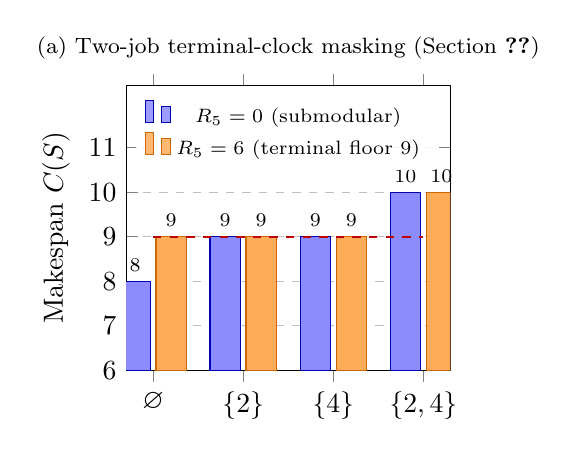
\begin{tikzpicture}
\begin{axis}[
    width=0.47\textwidth,
    height=5.2cm,
    ybar,
    bar width=11pt,
    ymin=6, ymax=12.4,
    ytick={6,7,8,9,10,11},
    ylabel={Makespan $C(S)$},
    symbolic x coords={S0, S2, S4, S24},
    xtick=data,
    xticklabels={{$\varnothing$}, {$\{2\}$}, {$\{4\}$}, {$\{2,4\}$}},
    legend style={at={(0.03,0.97)},anchor=north west,font=\scriptsize,draw=none,fill=white,fill opacity=0.85,text opacity=1},
    title={\footnotesize (a) Two-job terminal-clock masking (Section~\ref{sec:hardness})},
    nodes near coords,
    every node near coord/.append style={font=\scriptsize},
    ymajorgrids=true,
    grid style=dashed,
]
\addplot[fill=blue!45!white,draw=blue!70!black] coordinates {(S0,8) (S2,9) (S4,9) (S24,10)};
\addplot[fill=orange!65!white,draw=orange!80!black] coordinates {(S0,9) (S2,9) (S4,9) (S24,10)};
\draw[red!75!black,dashed,thick] (axis cs:S0,9) -- (axis cs:S24,9);
\legend{$R_5=0$ (submodular), $R_5=6$ (terminal floor $9$)}
\end{axis}
\end{tikzpicture}
\hfill
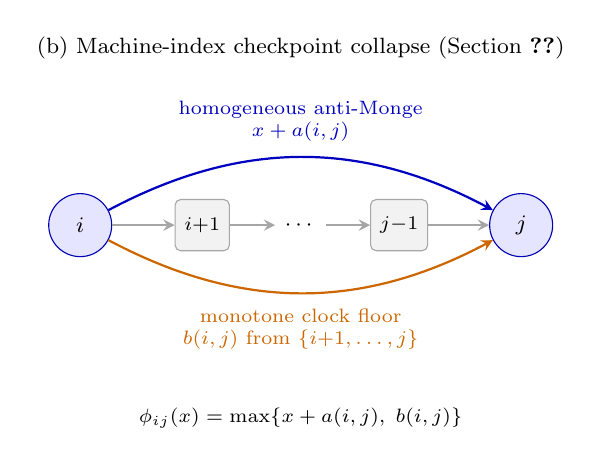
\begin{tikzpicture}[
    node distance=1.45cm,
    ckpt/.style={circle,draw=blue!70!black,fill=blue!10,minimum size=8mm,font=\footnotesize\bfseries},
    open/.style={rectangle,draw=gray!70,fill=gray!10,rounded corners=2pt,minimum size=6.5mm,font=\scriptsize},
    arr/.style={->,>=stealth,thick}
]
\node at (2.8,2.65) {\footnotesize (b) Machine-index checkpoint collapse (Section~\ref{sec:recurrence})};
\node[ckpt] (i) at (0,0.4) {$i$};
\node[open] (i1) at (1.55,0.4) {$i{+}1$};
\node[font=\footnotesize] (dots) at (2.8,0.4) {$\cdots$};
\node[open] (j1) at (4.05,0.4) {$j{-}1$};
\node[ckpt] (j) at (5.6,0.4) {$j$};
\draw[arr,gray!70] (i) -- (i1);
\draw[arr,gray!70] (i1) -- (dots);
\draw[arr,gray!70] (dots) -- (j1);
\draw[arr,gray!70] (j1) -- (j);
\draw[arr,blue!75!black,bend left=28] (i) to node[above,yshift=2pt,font=\scriptsize,align=center] {homogeneous anti-Monge\\$x + a(i,j)$} (j);
\draw[arr,orange!80!black,bend right=28] (i) to node[below,yshift=-2pt,font=\scriptsize,align=center] {monotone clock floor\\$b(i,j)$ from $\{i{+}1,\ldots,j\}$} (j);
\node[font=\scriptsize,align=center] at (2.8,-2.05) {$\phi_{ij}(x) = \max\{x + a(i,j),\; b(i,j)\}$};
\end{tikzpicture}
\caption{Core structural mechanisms: (a) delaying only the terminal machine's availability ($R_5=6$) lifts the baseline from $8$ to $9$, concealing both singleton increases while leaving the joint increase positive; (b) rank-one synchronization at consecutive selected machines $i<j$ collapses intervening open-mode machines into an anti-Monge homogeneous shift $a(i,j)$ and a predecessor-monotone clock floor $b(i,j)$.}
\label{fig:mechanism}
\end{figure}

\section{Certified Approximation with a Bound on Baseline Slack}
\label{sec:approx}

\begin{theorem}
\label{thm:approx}
For $0<\eta<1$, a feasible set and bounds $L\le\Delta^*\le U$ can be obtained with $O(m^2n+m^5/\eta)$ arithmetic operations. If an optimizing source has baseline slack at most $\rho\Delta^*$ and a bound $\rho$ is given, then choosing $\eta=\varepsilon/(1+\rho)$ guarantees $L\ge(1-\varepsilon)\Delta^*$. The running time is polynomial in the numerical value of $1+\rho$ and in $1/\varepsilon$. When job arrivals dominate the contribution of every machine clock for every feasible set, the job-arrival source suffices and yields an FPTAS.
\end{theorem}

\begin{proof}
External inputs comprise the original job release vector and the individual machine clocks. Let $C_h(S)$ be the makespan contribution when source $h$ is retained and the other absolute inputs are set to $-\infty$. For a machine clock the output where it enters is $R_h+P_h$, irrespective of that machine's mode. Use $h$ as a zero-cost start at $R_h$. Choices at $h$ and earlier cannot affect this contribution, so only its suffix is needed. From each source, the remaining homogeneous recurrence uses the precomputed graph, retaining subsequent compulsory positions and the free terminal sink. Max-plus superposition gives $C(S)=\max_h C_h(S)$. Define $\delta_h=C(\varnothing)-C_h(\varnothing)$ and $G_h=\max_S[C_h(S)-C_h(\varnothing)]$. Then $\Delta^*=\max_h(G_h-\delta_h)$.

For source $h$, let $q_h(j)$ be the start at $j$ with only mandatory predecessors and $j$ selected. Reweight an edge $i\to j$ as $q_h(i)+a(i,j)-q_h(j)$. It is nonnegative because an extra no-idle requirement cannot accelerate a completion. Telescoping shows that the path reward equals the increase from the source's own baseline. Remove edges whose two endpoints together exceed budget. Every remaining edge can be completed to a feasible path by retaining only its endpoints and compulsory vertices. With $M_h$ the maximum retained edge reward and $\ell_h$ an upper bound on path length, this gives $M_h\le G_h\le\ell_h M_h$. When $M_h>0$, floor each edge reward in units of $\eta M_h/\ell_h$. For each position and rounded reward, use a dynamic program to store minimum cost and a predecessor. Recover a witness at the largest affordable rounded reward. The loss is at most $\eta M_h$ and the rounded optimum plus $\ell_h$ units gives an upper bound. If $M_h=0$, the contribution cannot increase. Re-evaluate each witness under the original physical recurrence, keeping the best as $L$. Subtract $\delta_h$ from each source upper bound and take their maximum as $U$. For an optimizing source, $L\ge G_h-\delta_h-\eta G_h$. The claimed relative bound follows using $G_h=\Delta^*+\delta_h$. Each source has $O(m^2)$ edges and $O(m^2/\eta)$ rounded reward values, and there are at most $m+1$ sources.
\end{proof}

The result also gives the posterior certificate $L\ge(1-\varepsilon)U$ when this inequality happens to hold. The theorem supplies a running time for a known bound on the slack of an optimizing source. Detecting whether that promise holds is a separate question. For immediate machine availability, nonnegative job releases, and zero first setup on every machine, the job-arrival source dominates the machine clocks for every choice of requirements. The full guarantee then applies with $\rho=0$.

\subsection{Absolute Makespan and Partial Baseline Subtraction}

Subtracting a fixed baseline leaves the optimizing machine set unchanged and changes the multiplicative approximation guarantee. Let $C_{\mathrm{base}}=C(\varnothing)$ and $F_\lambda(S)=C(S)-\lambda C_{\mathrm{base}}$ for $0\le\lambda\le 1$. This interpolates between absolute makespan and the net increase. The relative loss is the reference-value deviation of \citet[][\S1]{Cornuejols1977} with reference $\lambda C_{\mathrm{base}}$.

\begin{corollary}
\label{cor:shifted}
Under the nonnegative timing assumptions of Section~\ref{sec:model}, absolute makespan and $F_\lambda$ for every fixed rational $0\le\lambda<1$ admit an FPTAS. For $F_\lambda$ the arithmetic bound is $O(m^2n+m^5/[\varepsilon(1-\lambda)])$. If $\lambda<1$ is part of the input in binary, no polynomial-time algorithm guarantees any fixed approximation factor unless $P=NP$, even when all feasible shifted scores are strictly positive and there are only two jobs and no setups.
\end{corollary}

\begin{proof}
Let $C^*=\max_S C(S)$ and choose an optimizing source $h$. Then $C^*=C_h(\varnothing)+G_h$. Every physical source in Section~\ref{sec:model} starts from nonnegative times and has nonnegative baseline completion. Thus $G_h\le C^*$. The source procedure from Theorem~\ref{thm:approx}, before subtracting source slack, returns a feasible set whose absolute makespan is at least $C^*-\eta G_h\ge(1-\eta)C^*$. Taking the best such set also works when $C^*=0$. Because $C_{\mathrm{base}}\le C^*$, the shifted optimum is at least $(1-\lambda)C^*$. Set $\eta=\varepsilon(1-\lambda)$. The same absolute error is then at most an $\varepsilon$ fraction of the shifted optimum. Path weights are sums and differences of the input times. Exact rational rounding uses polynomial bit length, and the rounded state count is polynomial in $1/\eta$. This also gives an FPTAS on input families with an inverse-polynomial lower bound on $1-\lambda$.

For the lower bound, fix an approximation factor $\gamma\ge 1$, with guarantee $F_\lambda(S)\ge\max_T F_\lambda(T)/\gamma$. Use the two-job instances from Theorem~\ref{thm:hardness}. The actual masked baseline $C_{\mathrm{base}}$ is a positive integer, and the optimal net increase is either zero or at least one. Choose $k$ so that $2^k>2\gamma C_{\mathrm{base}}$ and take the dyadic $\lambda=1-2^{-k}$. Its binary length is polynomial. Every feasible score is at least $b=2^{-k}C_{\mathrm{base}}>0$. If the increase is zero, every score is exactly $b$. If the increase is at least one, a $\gamma$-approximation must exceed $b$ because $(b+1)/\gamma>b$. Evaluating the returned set and testing $C(S)>C_{\mathrm{base}}$ would decide the NP-complete problem.
\end{proof}

A fixed time origin is part of the multiplicative guarantee for $\lambda<1$. A common shift of all times by $t$, when allowed by the model, adds $(1-\lambda)t$ to all shifted scores. The fully baseline-relative objective at $\lambda=1$ is invariant to that shift.

\section{When Is Timing Information Dispensable?}
\label{sec:deletion}

An input reduction can preserve every intermediate completion, or preserve only the final makespan used in the stress test. These criteria differ. We first hold the absolute time origin and the retained availability dates fixed and give a pair of results for terminal makespan. The Technical Appendix treats operation-level dates and the stronger guarantee on all completion times.

\begin{theorem}
\label{thm:deletion_hard}
For two jobs with zero setups, zero job release dates, and no compulsory no-idle machines, deciding whether deleting the first machine's initial availability time preserves the makespan for every budget-feasible set is weakly coNP-complete when the only other nonzero availability time is on the final machine.
\end{theorem}

\begin{proof}
From Theorem~\ref{thm:hardness}, the instance without absolute clocks has makespan $C_0+\sum_{i\in S}v_i$ for a feasible item selection $S$. Set the first machine's availability to $K=1+\sum_i v_i$. Set the terminal machine's availability to $H-P_m(2)$ for $H=C_0+K+T-1$, where $T\ge 1$ is the integer target profit. The terminal availability is nonnegative and the first availability is strictly positive. The terminal floor is $H$. With the first clock deleted, the unmasked makespan is less than $H$ for every feasible set, so the observed makespan is always $H$. With the first clock present, its delay shifts the entire unmasked schedule by $K$, so the observed makespan is $\max(H,C_0+K+\sum_{i\in S}v_i)$. A change is possible if and only if a feasible selection reaches target $T$. Such a change can be certified by a single lock set and two fixed-permutation simulations. Finally, for any instance in the stated class, write $F(S)$ for the makespan with both clocks removed and $H$ for the final machine floor. The clock is safe to delete if and only if $\max_S F(S)\le H-K$, which can be tested by the exact pseudo-polynomial budget recurrence. This proves the weak classification.
\end{proof}

\subsection{Removing a Downstream Suffix}

\begin{theorem}
\label{thm:suffix}
Suppose all initial machine availability dates on a specified suffix are removed together, and all earlier dates and the original job release dates are kept. The largest makespan error over feasible sets is achieved by the compulsory-only set or by a single affordable additional no-idle machine. The value and a witness can be found in $O(mn)$ time.
\end{theorem}

\begin{proof}
By superposition, if a selection $S$ has positive makespan error, a removed source at $h$ attains that error relative to the reduced schedule. Let $j\ge h$ be the first no-idle machine at or after $h$, using the final machine as a free no-idle sink. The isolated removed source and the reduced schedule have the same completion profile at $j$, up to their starting-time difference. All remaining absolute clocks were removed from the reduced suffix, so its propagation after $j$ is homogeneous. Thus the starting-time difference at $j$ equals the terminal error. Keep the compulsory set and $j$, dropping all other optional selections. This leaves the source contribution at $j$ unchanged since the machines between $h$ and $j$ remain open. The reduced start at $j$ can only decrease. Hence this empty or singleton selection witnesses an error at least as large.

Scan the two compulsory-only schedules, with and without the clock suffix. At a compulsory machine, the free terminal sink, or a machine whose cost lies within the budget, compare the two starts that would apply if that machine were locked. A positive difference is a lower bound on the error of that witness because the reduced suffix is homogeneous after the removal cut. Before the cut the two schedules agree. Taking the largest such difference attains the upper bound implied by the preceding witness argument. Each machine takes $O(n)$ work. Removal means using $-\infty$ for the deleted local terms. If a separate zero-time lower bound is retained, it is a retained clock and must satisfy the same placement assumptions.
\end{proof}

Applying Theorem~\ref{thm:suffix} with the suffix beginning at the first machine tests whether job arrivals alone preserve every feasible makespan. A zero maximum error establishes the single-source condition in Theorem~\ref{thm:approx}. The proof also applies to the operation-level timing inputs defined in the Technical Appendix because their isolated contributions enter before the first selected machine and the reduced suffix is homogeneous. The broader operation-level test was checked by enumeration on 1,906 budget-and-cut queries. Appendix~E extends the suffix singleton test to general max-plus switches with a sharp additive guarantee given by the largest projective diameter of an eligible switch. Appendix~F supplies a budget-sensitive upper bound for arbitrary clock deletion and certifies exactness when it meets the best singleton error.

\section{Fixed-Order Computational Comparison}
\label{sec:computational}

We compared exact algorithms for a given permutation on five deliberately truncated public processing-time matrices and four synthetic matrices, with experimental machine costs. Timings were taken in a pinned single-core Linux Python process with three timings per condition. The job-position dynamic program caches its within-machine prefix operations. All methods amortize the maximum-budget frontier when the cost vector is held fixed across a budget sweep. Table~\ref{tab:speedups} and Figure~\ref{fig:computational} report the median of the nine per-matrix CPU-time ratios, including initial graph construction. Independent checks covered all 54 distinct queries.


\begin{figure}[t]
\centering
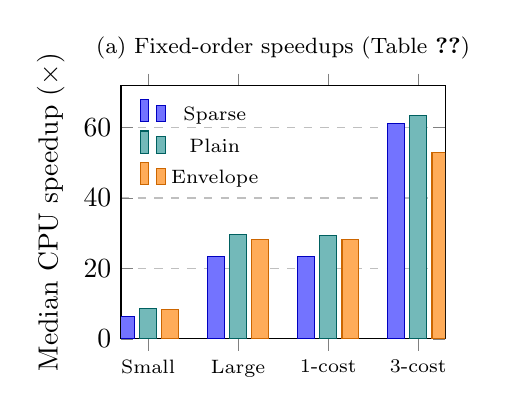
\begin{tikzpicture}
\begin{axis}[
    width=0.47\textwidth,
    height=4.8cm,
    ybar,
    bar width=6pt,
    ymin=0, ymax=72,
    ylabel={Median CPU speedup ($\times$)},
    symbolic x coords={Small, Large, Sweep, 3-Cost},
    xtick=data,
    xticklabels={Small, Large, 1-cost, 3-cost},
    xticklabel style={font=\scriptsize},
    legend style={at={(0.03,0.97)},anchor=north west,font=\scriptsize,draw=none,fill=none},
    title={\footnotesize (a) Fixed-order speedups (Table~\ref{tab:speedups})},
    ymajorgrids=true,
    grid style=dashed,
]
\addplot[fill=blue!55!white,draw=blue!75!black] coordinates {(Small,6.39) (Large,23.43) (Sweep,23.41) (3-Cost,61.27)};
\addplot[fill=teal!55!white,draw=teal!75!black] coordinates {(Small,8.58) (Large,29.56) (Sweep,29.43) (3-Cost,63.46)};
\addplot[fill=orange!65!white,draw=orange!80!black] coordinates {(Small,8.46) (Large,28.31) (Sweep,28.26) (3-Cost,53.00)};
\legend{Sparse, Plain, Envelope}
\end{axis}
\end{tikzpicture}
\hfill
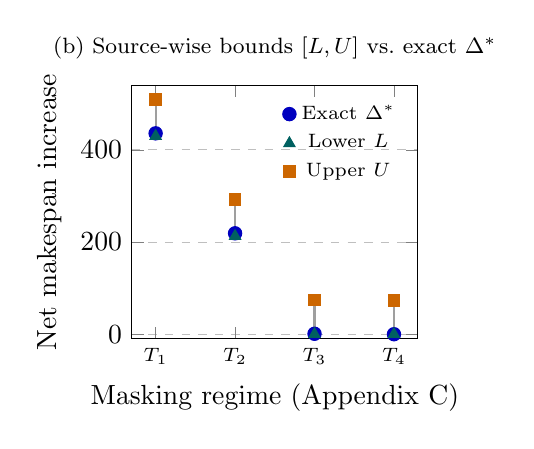
\begin{tikzpicture}
\begin{axis}[
    width=0.43\textwidth,
    height=4.8cm,
    ymin=-10, ymax=540,
    ylabel={Net makespan increase},
    xlabel={Masking regime (Appendix~C)},
    xtick={1,2,3,4},
    xticklabels={$T_1$, $T_2$, $T_3$, $T_4$},
    xticklabel style={font=\scriptsize},
    legend style={at={(0.97,0.97)},anchor=north east,font=\scriptsize,draw=none,fill=none},
    title={\footnotesize (b) Source-wise bounds $[L,U]$ vs.\ exact $\Delta^*$},
    ymajorgrids=true,
    grid style=dashed,
]
\addplot[only marks,mark=*,mark size=2.4pt,blue!75!black] coordinates {(1,436) (2,219) (3,1) (4,0)};
\addplot[only marks,mark=triangle*,mark size=2.3pt,teal!75!black] coordinates {(1,430) (2,213) (3,0) (4,0)};
\addplot[only marks,mark=square*,mark size=2.1pt,orange!80!black] coordinates {(1,509) (2,292) (3,74) (4,73)};
\draw[gray!75,thick] (axis cs:1,430) -- (axis cs:1,509);
\draw[gray!75,thick] (axis cs:2,213) -- (axis cs:2,292);
\draw[gray!75,thick] (axis cs:3,0) -- (axis cs:3,74);
\draw[gray!75,thick] (axis cs:4,0) -- (axis cs:4,73);
\legend{Exact $\Delta^*$, Lower $L$, Upper $U$}
\end{axis}
\end{tikzpicture}
\caption{Empirical evidence from archived experiments: (a) median paired CPU speedups of machine-state recurrences over job-position dynamic programming across nine fixed-order matrices, including preprocessing; (b) certified Theorem~\ref{thm:approx} intervals $[L,U]$ at $\eta=1/4$ as a terminal clock masks true net increase $\Delta^*\in\{436,219,1,0\}$ (Appendix~C).}
\label{fig:computational}
\end{figure}

These measurements evaluate the sparse, plain, and binary-search implementations. The online linear-time matrix search in Theorem~\ref{thm:exact} is a theoretical bound. The binary-search envelope was slower than the plain machine recurrence on all nine matrices in the three-cost batch. The speedups support repeated fixed-order scoring on the tested sizes. In a separate downstream permutation-search experiment comparing the same screened search under machine-state versus job-position scoring, mean reductions in final worst-case makespan were $0.239\%$ at $0.15$ CPU seconds and $0.109\%$ at $0.45$ CPU seconds per instance, both below the prespecified $1\%$ threshold. The Technical Appendix gives additional timing details and the scope of those experiments.

\section{Discussion}
\label{sec:discussion}

A single terminal availability date can set a floor on the baseline makespan and hide upstream delays until the added no-idle requirements lift completion above it, bridging the gap between a tractable homogeneous flow-shop subclass and the general-network differential inapproximability barrier. For fixed-order no-idle stress tests, the machine-index recurrence decouples job count from budget queries, and the suffix test certifies in linear time whether downstream timing information is dispensable for the final makespan---and whether the single-source FPTAS applies. For arbitrary deletion, the Technical Appendix gives an exact budget-dependent oracle and shows that preserving only the final makespan changes the complexity of finding a smallest retained clock set. Our computational evidence concerns controlled public processing-time prefixes and synthetic schedules; plant-floor datasets and substantial improvements in outer permutation optimization remain outside the scope established here.

\section*{Code and Data Availability}

The supplementary archive contains a Python reference implementation and computational checks. Its README gives instructions for locating the inputs and replaying the fixed-order timing comparison. The five public processing-time inputs come from the \href{https://huggingface.co/datasets/frontieror/FrontierOR/tree/ef42a2eac13595453f986d9df0b62e86e75ab596/tasks/ruiz2007}{FrontierOR Ruiz task at the archived revision}. The synthetic inputs are generated from fixed seeds.

\section*{Acknowledgments}

Google Antigravity and OpenAI Codex assisted with research development, including hypothesis development, implementation, computational analysis, and manuscript drafting.

\clearpage
\bibliographystyle{plainnat}
\bibliography{references}

\clearpage
\begin{table}[!ht]
\centering
\footnotesize
\caption{Structural separation between general budgeted project interdiction and fixed-order mixed no-idle flow shops.}
\label{tab:separation}
\begin{tabularx}{\textwidth}{>{\raggedright\arraybackslash}p{2.6cm}>{\raggedright\arraybackslash}X>{\raggedright\arraybackslash}X>{\raggedright\arraybackslash}X}
\toprule
Problem aspect & General budgeted project DAG \citep{Brown2005,Wu2026} & Fixed-order flow shop without active clocks ($R_i=0$, $s_i(1)=0$, $r_t\ge 0$) & Fixed-order flow shop with availability dates ($R_i\ge 0$, arbitrary $r_t, s_i$) \\
\midrule
Exact evaluation (heterogeneous integer costs) & $O(mn^2(B+1))$ generic; $O(mn(B+1))$ using within-machine separability & $O(m^2n)$ prep.\ + $O(m(B+1)\log(m+1))$ (theoretical $O(m(B+1))$, Theorem~\ref{thm:exact}) & Same bound via anti-Monge $a(i,j)$ + monotone $b(i,j)$ (Lemmas~\ref{lem:monge}--\ref{lem:monotone}, Theorem~\ref{thm:exact}) \\
\addlinespace[4pt]
Deciding $\Delta^*>0$ and differential approximation & Weakly NP-complete even with zero external clocks; no finite-factor approx.\ unless $P=NP$ & Monotone submodular; $O(mn)$ singleton check (Corollary~\ref{cor:submod}) and differential FPTAS (Theorem~\ref{thm:approx}, $\rho=0$) & Weakly NP-complete with one terminal clock $R_m>0$ and $n=2$ (Theorem~\ref{thm:hardness}); $(1-\varepsilon)$-approx.\ in $\mathrm{poly}(m, 1+\rho, 1/\varepsilon)$ (Theorem~\ref{thm:approx}); FPTAS for $F_\lambda$ at fixed $\lambda\in[0,1)$ but no fixed factor for binary-input $\lambda<1$ (Corollary~\ref{cor:shifted}) \\
\addlinespace[4pt]
All-completions clock reduction & Not covered by project-interdiction evaluation models & Trivial (all local clocks redundant) & Minimum-cardinality local-bound support in $O(mn)$ time (Proposition~A.1) \\
\addlinespace[4pt]
Downstream suffix deletion (makespan error) & Parallel bypasses prevent singleton collapse & All clocks dispensable ($0$ error) & Exact max error by $\varnothing$ or singleton in $O(mn)$ time; certifies $\rho=0$ FPTAS (Theorem~\ref{thm:suffix}); extends to switched max-plus cascades up to projective diameter $D_{\max}$ (Proposition~E.1) \\
\addlinespace[4pt]
Arbitrary clock deletion (makespan invariance) & Not covered by project-interdiction evaluation models & Trivial ($0$ error) & Weakly coNP-complete even for $n=2$ with two clocks (Theorem~\ref{thm:deletion_hard}); $O(m(B+1)\log(m+1))$ uniform-threshold oracle (Appendix~B); Lagrangian budget certificate (Proposition~F.1) \\
\addlinespace[4pt]
Minimum clock retention (tolerance $\varepsilon$) & Not covered by project-interdiction evaluation models & $0$ clocks required & Exact cut generation (Appendix~B); factor-$2$ inapproximability even with $n=2$ and two clocks (Proposition~7) \\
\bottomrule
\end{tabularx}
\end{table}

\begin{table}[!ht]
\centering
\small
\caption{Median paired CPU speedups over job-position dynamic programming across nine fixed-order matrices (including preprocessing).}
\label{tab:speedups}
\begin{tabular}{lrrr}
\toprule
Query workload & Sparse states & Plain states & Binary-search envelope \\
\midrule
Cold, smallest budget & $6.39\times$ & $8.58\times$ & $8.46\times$ \\
Cold, largest budget & $23.43\times$ & $29.56\times$ & $28.31\times$ \\
Several budgets, one set of costs & $23.41\times$ & $29.43\times$ & $28.26\times$ \\
All budgets, three sets of costs & $61.27\times$ & $63.46\times$ & $53.00\times$ \\
\bottomrule
\end{tabular}
\end{table}

\end{document}
